\chapter{Wdrażanie systemu} \label{chapter_deployment}

% Napisać jeszcze raz, wtf
Jak zaznaczono~w zakresie pracy (\ref{intro_objective}),
architektura systemu ma pozwalać na automatyzację wdrożeń.
W niniejszym rozdziale opisane są technologie~i praktyki, które zostały 
zastosowane, aby zautomatyzować wdrażanie systemu.

\section{Konteneryzacja}

Wszystkie elementy systemu (za wyjątkiem oprogramowania na dronie) są uruchamiane~w kontenerach.
Wykorzystanym systemem konteneryzacji jest \texttt{docker}\cite{docker}.
Konteneryzacja pozwala na zupełne zautomatyzowanie
procesu budowania oprogramowania~i instalacji koniecznych
składników środowiska uruchomieniowego. Aby zbudować kontener zawierający
aplikację, programista musi napisać skrypt,~w wyniku
którego~w kontenerze zostanie zainstalowane konieczne 
do uruchomienia aplikacji oprogramowanie. Proces instalacji~i konfiguracji
wymaganych bibliotek jest więc automatyczny~i deterministyczny -- wszystko
zależy tylko~i wyłącznie od skryptu budującego kontener.

Konteneryzacja ułatwia proces przenoszenia oprogramowania~z maszyny na maszynę. Raz zbudowany
kontener może zostać uruchomiony na dowolnej nowej maszynie, bez konieczności instalowania 
czy konfigurowania bibliotek czy programów. 

\subsection{Zachowywanie stanu systemu plików~w kontenerze} \label{volumes}

Ważną różnicą, jaka odróżnia kontenery od aplikacji zainstalowanych~w sposób konwencjonalny, jest \textbf{bezstanowość}. Jeśli komputer,
na którym działają kontenery zostanie zresetowany, bądź kontener zostanie
usunięty~i utworzony na nowo (na przykład~w celu aktualizacji), system
plików~w kontenerze zostanie zresetowany do stanu,~w jakim znajdował się ~w momencie uruchomienia (takim, jaki jest zapisany~w \textit{obrazie kontenera}).

\texttt{Docker} pozwala rozwiązać ten problem za pomocą mechanizmu 
woluminów (\textit{docker volumes})\cite{docker_volumes}.
Za pomocą woluminów, dowolny fragment systemu
plików kontenera może zostać zmapowany do nieulotnej pamięci komputera, na którym 
działa kontener.~W ten sposób zapewnia się persystencję baz danych lub innych
plików, które mają być przechowywane przez aplikację.\\ % newline CAN be removed

\textit{Uwaga:} nie wszystkie kontenery potrzebują zachowywać pliki -- kontener
odpowiedzialny za hostowanie statycznej strony internetowej nie potrzebuje
zapamiętywać zmian, ponieważ pliki strony nie zmieniają się podczas hostowania. 

\section{Automatyczne budowanie~i testowanie komponentów systemu}

Jak wspomniano~w rozdziale \ref{repo_structure}, poświęconym strukturze repozytoriów,
wszystkie repozytoria zawierają plik \texttt{.gitlab-ci.yml}. Plik ten definiuje skrypty,
jakie wykona potok \texttt{CI/CD}, gdy do repozytorium zostanie dodany nowy kod.
Diagram ilustrujący proces pracy programisty~z potokiem \textit{CI/CD} zawarty jest
na rysunku \ref{ci_workflow}.

\begin{figure}[H]
	\centering\small

\tikzstyle{arrow} = [thick,->,>=stealth]
\begin{tikzpicture}[node distance=4cm,auto,>=stealth']
    
    \node[] (programmer) {Programista};
    \node[right of = programmer] (repo) {Repozytorium};
    \node[right of = repo] (ci_cd) {Potok \texttt{CI/CD}};
    \node[right of = ci_cd] (registry) {Rejestr kontenerów};

    \node[below of = programmer, node distance=6cm] (programmer_ground) {};
    \node[below of = repo, node distance=6cm] (repo_ground) {};
    \node[below of = ci_cd, node distance=6cm] (ci_cd_ground) {};
    \node[below of = registry, node distance=6cm] (registry_ground) {};
    %
    \draw (repo) -- (repo_ground);
    \draw (programmer) -- (programmer_ground);
    \draw (ci_cd) -- (ci_cd_ground);
    \draw (registry) -- (registry_ground);


    \draw[->] ($(programmer)!0.20!(programmer_ground)$) -- node[above,scale=1,midway]{Nowy \textit{commit}} ($(repo)!0.20!(repo_ground)$);
    % \draw[<-] ($(programmer)!0.35!(programmer_ground)$) -- node[above,scale=1,midway]{Text} ($(repo)!0.35!(repo_ground)$);
    \draw[->,align=center] ($(repo)!0.35!(repo_ground)$) -- node[above,scale=1,midway]{Zainicjowanie procesu\\budowania} ($(ci_cd)!0.35!(ci_cd_ground)$);

    \draw[->,align=center] ($(ci_cd)!0.60!(ci_cd_ground)$) -- node[above,scale=1,midway]{ Wysłanie zbudowanego \\~i przetestowanego \\ konteneru do rejestru} ($(registry)!0.60!(registry_ground)$);
    
    \draw[<-,align=center] ($(repo)!0.70!(repo_ground)$) -- node[above,scale=1,midway]{Status~i logi \\z potoku \texttt{CI/CD}} ($(ci_cd)!0.70!(ci_cd_ground)$);
    \draw[<-,align=center] ($(programmer)!0.90!(programmer_ground)$) -- node[above,scale=1,midway]{Informacja, czy \\ \textit{commit} przeszedł testy} ($(repo)!0.90!(repo_ground)$);
\end{tikzpicture}
	\caption{
      Diagram sekwencji, opisujący proces automatycznej budowy i testowania kontenerów 
	}
	\label{ci_workflow}
\end{figure}

Ponieważ konteneryzacja pozwala na zupełne zautomatyzowanie procesu budowania,
skrypty~w potoku \texttt{CI/CD} są~w stanie samodzielnie zbudować kontener,
zawierający konkretny komponent systemu. Następnie, kontener poddawany jest testom
(opisanym~w rozdziale \ref{chapter_tests}). Po przejściu testów, kontener wysyłany jest
do \textit{rejestru kontenerów} -- specjalnego repozytorium, w~którym można
przechowywać~i wersjonować kontenery. Skrypt potoku \texttt{CI/CD} automatycznie oznacza
kontener za pomocą nazwy brancha, na której został zbudowany. Kontenery pochodzące~z brancha
\textit{master}, uruchamiane są na serwerze produkcyjnym. Przykładowa konfiguracja
\textit{Gitlab CI}, wykorzystywana~w repozytorium aplikacji klienckiej opisana została~w listingu
\ref{list:ci_cd_frontend}.

\begin{lstlisting}[language=yml, label=list:ci_cd_frontend,caption={Plik konfiguracyjny \textit{Gitlab CI}, budujący aplikację kliencką }, basicstyle=\footnotesize\ttfamily]
# Definicje zmiennych, wpływających na proces budowania
variables:
  # Wywołuje automatyczne pobranie submodułów,
  # przed przystąpieniem do budowania 
  GIT_SUBMODULE_STRATEGY: recursive
 
  # Zapewnia dostęp do dockera z poziomu systemu CI/CD
  DOCKER_HOST: tcp://docker:2375
  DOCKER_TLS_CERTDIR: "" 

  # Specyfikuje nazwę kontenera, który zostanie zbudowany 
  IMAGE_NAME: "registry.gitlab.com/academic-aviation-club/gavron/frontend"

# Przed wykonaniem danego skryptu budującego, wykonywane jest logowanie
# do rejestru dockera - umożliwi to zapisanie w nim 
# zbudowanego obrazu aplikacji. Zmienna $GITLAB_DEPLOY_TOKEN
# przypisywana jest w ustawieniach repozytorium
before_script:
  - docker login -u baczek-vps -p $GITLAB_DEPLOY_TOKEN registry.gitlab.com

# Zawsze budowany jest obraz testowy, który zostanie
# później wykorzystany do testów systemowych 
build_testing_image:
  stage: build
  # Zapewnia dostęp do dockera w ramach zadania `build_testing_image`
  services:
    - docker:19.03.12-dind
  image: docker:19.03.12
  
  # Skrypt wpierw buduje obraz dockera, zawierający aplikację.
  # Następnie uruchamia na obrazie testy jednostkowe. Jeśli testy
  # nie zwrócą błędu, obraz jest wysyłany do rejestru.
  # Na obrazach w rejestrze wykonywane są testy systemowe.
  script:
  - docker build -f docker/test.dockerfile -t $IMAGE_NAME:test_$CI_COMMIT_REF_NAME .
  - docker run $IMAGE_NAME:$CI_COMMIT_REF_NAME "npm run test"
  - docker push $IMAGE_NAME:test_$CI_COMMIT_REF_NAME

# Tylko dla brancha `master`, budowany jest obraz 
# produkcyjny, który zostanie uruchomiony na serwerze
build_prod_image:
  stage: build
  services:
	- docker:19.03.12-dind	
  # `only` pozwala na wybranie brancha, na którym działa dany skrypt
  only:
    - master
  image: docker:19.03.12
   
  script:
  - docker build -f docker/Dockerfile -t $IMAGE_NAME:$CI_COMMIT_REF_NAME .
  - docker run $IMAGE_NAME:$CI_COMMIT_REF_NAME "npm run test"
  - docker push $IMAGE_NAME:$CI_COMMIT_REF_NAME
\end{lstlisting}

Wszystkie logi, jakie potok CI/CD zbierze~w trakcie budowania~i testowania obrazu~z aplikacją są
dostępne dla programisty -- pozwala to odnaleźć błędy, które pojawiły się~w procesie budowania oraz
sprawdzić wyniki testów. Systemy obsługi repozytorium (taki jak \textit{GitHub}, \textit{BitBucket}
czy \textit{GitLab}), wyświetlają informacje~o tym, czy dany commit przeszedł testy~w potoku 
\textit{CI/CD}, ułatwiając odnajdywanie commitów zawierających błędy. Przykład tej funkcji
zilustrowany jest na rysunku \ref{gitlab_ci_history}.

\begin{figure}[H]
  \centering
  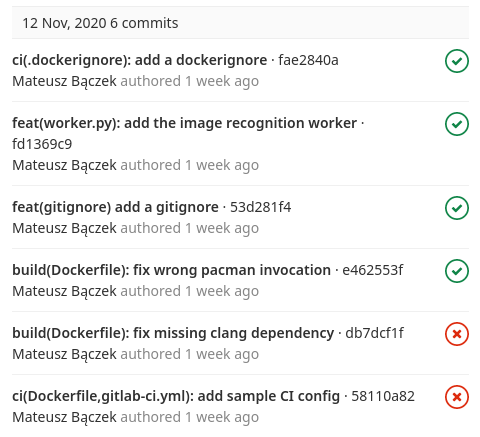
\includegraphics[width=.7\linewidth]{rys04/gitlab_ci_commit_status.png}
  \caption{ Historia zmian~w kodzie~w serwisie \textit{GitLab}.
  Ikony po prawej stronie informują, czy dany commit przeszedł testy~w potoku CI/CD }
	\label{gitlab_ci_history}
\end{figure}

\section{Automatyczne aktualizacje kontenerów} \label{ouroboros}

Pobranie~i uruchomienie kontenera, zawierającego dany komponent systemu
nie wymaga przechodzenia przez proces instalacji czy konfiguracji -- wystarczy
pobrać obraz kontenera~z rejestru~i uruchomić go:

\begin{lstlisting}[language=bash, label=list:docker_clone_run_example,caption={Pobranie~i uruchomienie obrazu dockera, zawierającego aplikację}, basicstyle=\footnotesize\ttfamily]
# Zapisane jako zmienna, aby poprawić czytelność przykładu 
IMAGE=registry.gitlab.com/academic-aviation-club/gavron/frontend:master

docker pull $IMAGE
docker run \
    -d \ # detach: kontener działa w tle, nie wysyła logów do terminala
    -p 5000:5000 \ # mapuje port 5000 z kontenera do portu na komputerze  
    --name frontend \ # Nadaje nazwę uruchomionemu kontenerowi
    $IMAGE # Nazwa obrazu do uruchomienia 
\end{lstlisting}
~W przypadku, gdy na serwerze działa już kontener~z aplikacją, należy
pobrać nowy obraz kontenera, usunąc obecnie działający kontener~i uruchomić
nowy obraz:

\begin{lstlisting}[language=bash, label=list:docker_update_container,caption={Aktualizacja kontenerów}, basicstyle=\footnotesize\ttfamily]
IMAGE=registry.gitlab.com/academic-aviation-club/gavron/frontend:master

docker pull $IMAGE # Pobranie najnowszej wersji kontenera

# Nazwa kontenera nadana w poprzednim przykładzie, za pomocą --name
docker stop frontend

# Usunięcie kontenera w starej wersji (jego stanu, zmian w systemie plików)
docker rm frontend

# Tak samo jak w przykładzie powyżej
docker run \
    -d \ # detach: kontener działa w tle, nie wysyła logów do terminala
    -p 5000:5000 \ # mapuje port 5000 z kontenera do portu na komputerze  
    --name frontend \ # Nadaje nazwę uruchomionemu kontenerowi
    $CONTAINER # Nazwa kontenera do uruchomienia 
\end{lstlisting}
~W przypadku wielu równolegle działających kontenerów, ręczna aktualizacja 
każdej działającej aplikacji jest zadaniem niepotrzebnie czasochłonnym.
Wprowadza też dodatkowy punkt,~w którym może zajść pomyłka -- na przykład
pominięcie jednego~z kontenerów przy aktualizacji.

Projekt wykorzystuje narzędzie \texttt{Ouroboros} do automatycznej aktualizacji
uruchomionych na serwerze kontenerów. \texttt{Ouroboros}~w regularnych odstępach
czasu sprawdza, czy uruchomione na serwerze kontenery nie wymagają aktualizacji.
Jeśli~w rejestrze dostępna jest nowa wersja obrazu kontenera, pobiera ją~i zastępuje
nią obecnie działający kontener.

Dzięki zastosowaniu narzędzia \texttt{Ouroboros}, w trakcie testów w terenie 
udało się znacznie usprawnić aktualizacje infrastruktury systemu. W przypadku
pojawienia się błędu, programiści musieli jedynie zaktualizować kod w repozytorium --
potok \textit{CI/CD} automatycznie budował poprawioną wersję kontenera, \texttt{Ouroboros}
aktualizował serwer produkcyjny. Po dodaniu nowego kodu do repozytorium, uaktualniona
wersja aplikacji pojawiała się na serwerze po mniej niż pięciu minutach.

\section{Orkiestracja systemu złożonego~z wielu kontenerów -- \texttt{docker-compose}}

Finalnie, infrastruktura internetowa systemu składa się~z sześciu
jednocześnie działających kontenerów dockerowych:

\begin{enumerate}
  \item Kontener serwujący stronę internetową~z aplikacją kliencką,
  \item Kontener~z serwerem API,
  \item Kontener~z serwerem \texttt{imagezmq},
  \item Kontener~z systemem telemetrii,
  \item Kontener~z programem \texttt{ouroboros} (opisanym~w rozdziale \ref{ouroboros}),
  \item Kontener~z systemem do rozpoznawania obrazów. 
\end{enumerate}

\noindent
Każdy kontener musi zostać odpowiednio skonfigurowany~w momencie uruchamiania.
Konfiguracja poszczególnego kontenera obejmuje:

\begin{itemize}
  \item Przypisanie limitów zasobów (n.p. maksymalny procent wykorzystania procesora)
  \item Udostępnienie portów serwera, które może wykorzystywać dany kontener,
  \item Przypisanie woluminów systemu plików serwera,~w celu zapewnienia persystencji
        danych, zapisywanych przez kontener (opisane~w rozdziale \ref{volumes}),
  \item Zdefiniowanie reguł automatycznego restartu kontenera (na przykład gdyby proces
        działający~w kontenerze uległ awarii),
  \item Określenie zmiennych środowiskowych, które mogą wpływać na zachowanie się
        procesów wewnątrz kontenera (przykładowo, kontener \texttt{ouroboros} pozwala
        za pomocą zmiennych środowiskowych określić, jak często mają być sprawdzane
        aktualizacje kontenerów).
\end{itemize}

Narzędzie \texttt{docker-compose} pozwala zebrać całą konfigurację kontenerów do 
jednego pliku konfiguracyjnego \cite{docker_compose}.~W ten sposób, po uzyskaniu
dostępu do rejestru~z kontenerami, zawierającymi komponenty systemu, możliwe jest
natychmiastowe pobranie~i uruchomienie systemu~z właściwą konfiguracją kontenerów.

